\documentclass[10pt]{article}
\usepackage[polish]{babel}
\usepackage[utf8]{inputenc}
\usepackage[T1]{fontenc}
\usepackage{amsmath}
\usepackage{amsfonts}
\usepackage{amssymb}
\usepackage[version=4]{mhchem}
\usepackage{stmaryrd}
\usepackage{graphicx}
\usepackage[export]{adjustbox}
\graphicspath{ {./images/} }

\title{GIMNAZJUM }

\author{}
\date{}


\begin{document}
\maketitle
\begin{enumerate}
  \item ABCD jest czworokątem. Punkty K, L, M, N są środkami boków \(A B, B C, C D, D A\). Uzasadnij, że pole części zielonej jest takie samo, jak pole części niebieskiej.
  \item Wewnątrz trójkąta równobocznego \(A B C\) obrano dowolnie punkt P i zrzutowano go prostopadle na boki \(B C, C A\) i \(A B\), otrzymując w ten sposób odpowiednio punkty D, E i F. Udowodnij, że \(A F+B C+C E\) nie zależy od wyboru punktu P .
  \item Udowodnij, że jeżeli liczby \(a, b, c\) są dodatnie to \(a^{2}+b^{2}+c^{2} \geq a b+b c+c a\)\\
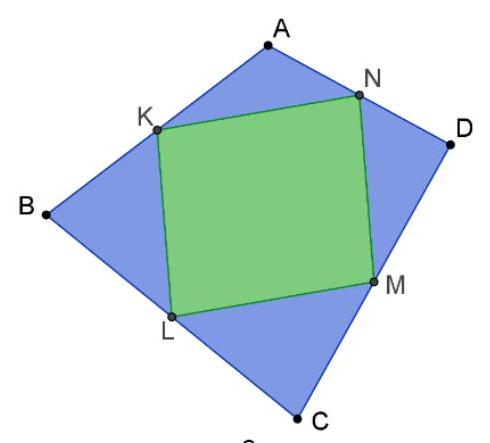
\includegraphics[max width=\textwidth, center]{2024_11_21_c35196432bacdc36866cg-1}
\end{enumerate}

\section*{LICEUM}
\begin{enumerate}
  \item Udowodnij, że dwusieczna kąta prostego w trójkącie prostokątnym dzieli kwadrat zbudowany na przeciwprostokątnej na dwie części o równych polach.
  \item Na przeciwprostokątnej \(A B\) równoramiennego trójkąta prostokątnego \(A B C\) obrano takie punkty K i L, że kąt KCL \(=45^{\circ}\). Udowodnij, że \(A K^{2}+L B^{2}=K L^{2}\).
  \item Udowodnij, że jeżeli liczby \(a, b, c\) są dodatnie i \(a b+b c+c a=1\) to \(a+b+c \geq \sqrt{3}\)
\end{enumerate}

\end{document}